\documentclass{lecture}

\usetikzlibrary{quotes,angles,babel}
\usepackage{bm}

\institute{Lehr- und Forschungsgebiet Kontinuumsmechanik}
\title{Vorlesung 1}
\author{Joshua Feld, 406718}
\course{Mechanik verformbarer Körper}
\professor{Itskov}
\semester{Sommersemester 2022}
\program{CES (Bachelor)}

\begin{document}
    \maketitle


    \section*{Spannungszustand}

    Die Intensität der inneren Kräfte wird in einem materiellen Köper durch die Spannungen charakterisiert.
    In einem geraden Stab bestimmt man dabei die Spannung als Verhältnis der axialen Kraft \(F\) zu der Querschnittsfläche \(A\)
    \begin{equation}\label{eq:1}
        \sigma = \frac{F}{A}.
    \end{equation}
    Dabei geht man von einer gleichmäßigen Verteilung der inneren Kräfte über den Querschnitt aus.
    Die Dimension der Spannung ist somit Kraft pro Fläche und wird üblicherweise in \(1\sis{\pascal} = 1\sis{\newton\per\meter\squared}\) oder \(1\sis{\mega\pascal} = 1\sis{\newton\per\milli\meter\squared}\) angegeben.
    \begin{center}
        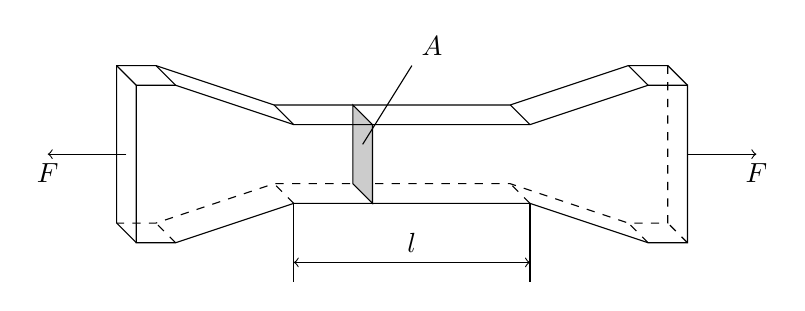
\begin{tikzpicture}
            \draw[dashed] (6.75,2.25) -- (6.75,.25) -- (6.25,.25) -- (4.75,.75) -- (1.75,.75) -- (.25,.25) -- (-.25,.25);
            \draw[fill=white!80!black] (3,.5) -- (2.75,.75) -- (2.75,1.75) -- (3,1.5) -- cycle;
            \draw (0,0) -- (0,2) -- (.5,2) -- (2,1.5) -- (5,1.5) -- (6.5,2) -- (7,2) -- (7,0) -- (6.5,0) -- (5,.5) -- (2,.5) -- (.5,0) -- cycle;
            \draw (-.25,.25) -- (-.25,2.25) -- (.25,2.25) -- (1.75,1.75) -- (4.75,1.75) -- (6.25,2.25) -- (6.75,2.25);
            \draw (0,2) -- (-.25,2.25);
            \draw (.5,2) -- (.25,2.25);
            \draw (2,1.5) -- (1.75,1.75);
            \draw (5,1.5) -- (4.75,1.75);
            \draw (6.5,2) -- (6.25,2.25);
            \draw (7,2) -- (6.75,2.25);
            \draw (0,0) -- (-.25,.25);
            \draw[dashed] (.5,0) -- (.25,.25);
            \draw[dashed] (2,.5) -- (1.75,.75);
            \draw[dashed] (5,.5) -- (4.75,.75);
            \draw[dashed] (6.5,0) -- (6.25,.25);
            \draw[dashed] (7,0) -- (6.75,.25);
            \draw[->] (-.125,1.125) -- (-1.125,1.125) node[below] {\(F\)};
            \draw[->] (7,1.125) -- (7.875,1.125) node[below] {\(F\)};
            \draw (2.875,1.25) -- (3.5,2.25) node[above right] {\(A\)};
            \draw (2,.5) -- (2,-.5);
            \draw (5,.5) -- (5,-.5);
            \draw[<->] (2,-.25) -- (5,-.25) node[midway,above] {\(l\)};
        \end{tikzpicture}
    \end{center}

    Im Gegensatz zu geraden Stäben kann man bei einem dreidimensionalen Körper im Allgemeinen nicht mehr von einer konstanten Spannungverteilung ausgehen.
    Somit gilt Beziehung \eqref{eq:1} nicht mehr.
    Die Bestimmung der Spannung basiert dabei auf der Theorie von Cauchy, die im Folgenden kurz erläutert wird.


    \section*{Spannungsvektor und Spannungstensor}

    Wir betrachten einen beliebigen Körper im dreidimensionalen Raum.
    In einem Punkt \(P\) dieses Körpers soll der komplette Spannungszustand erfasst werden.
    Damit sollen die Spannungen in allen Ebenen durch diesen Punkt bestimmt werden.

    % TODO: Bestimmung des Spannungsvektors

    Wir fangen mit einer beliebigen Ebene an.
    Diese Ebene schneidet einen Teil (links) des Körpers frei.
    Durch die Schnittfläche übt der andere Teil (rechts) bestimmte Kräfte aus, die im Allgemeinen ungleichmäßig über diese Fläche verteilt sind.
    Um die Spannung im Punkt \(P\) zu bestimmen, definieren wir zunächst eine kleine Teilfläche \(\Delta A\) um \(P\).
    Sei \(\Delta\mathbf{F}\) die Resultierende aller Kräfte, die auf dieser Teilfläche wirken.
    Durch den Quotienten \(\frac{\Delta\mathbf{F}}{\Delta A}\) bestimmt man die mittlere Spannung für das Flächenelement \(\Delta A\).
    Durch den Grenzübergang \(\Delta A \to 0\) wird der so genannte Cauchy'sche Spannungsvektor
    \begin{equation}\label{eq:2}
        \mathbf{t} = \lim_{\Delta A \to 0}\frac{\Delta\mathbf{F}}{\Delta A} = \frac{\d\mathbf{F}}{\d A}
    \end{equation}
    definiert.
    Die Voraussetzung, dass dieser Grenzvektor existiert und endlich ist, stellt eine fundamentale Annahme (Cauchy-Annahme) der Mechanik dar.

    Durch vektorielle Zerlegung lässt sich dieser Vektor in eine Komponente normal und in eine Komponente tangential zur Schnittfläche zerlegen.
    Dabei wird die normale Komponente als Normalspannung (\(\sigma\)) und die tangentiale als Schubspannung (\(\tau\)) bezeichnet.

    Der Spannungsvektor \(\mathbf{t}\) in einem Punkt hängt von der Richtung der Schnittfläche ab, die durch die äußere Normale \(\mathbf{n}\) festgelegt ist.
    Die Art dieser Abhängigkeit werden wir später untersuchen und feststellen.

    Durch den Spannungsvektor \(\mathbf{t}\) auf einer einzigen Schnittfläche wird der Spannungszustand im Punkt \(P\) allerdings nicht ausreichend beschrieben.
    Man kann allerdings zeigen, dass hierzu die Spannungsvektoren in drei senkrecht aufeinander stehenden Schnittflächen im Allgemeinen notwendig sind.
    Zur Bestimmung des Spannungszustandes schneiden wir daher gedanklich einen infinitesimalen Quader mit den Kantenlängen \(\d x\), \(\d y\) und \(\d z\) aus einem Körper, in direkter Umgebung zum Punkt \(P\).
    \begin{center}
        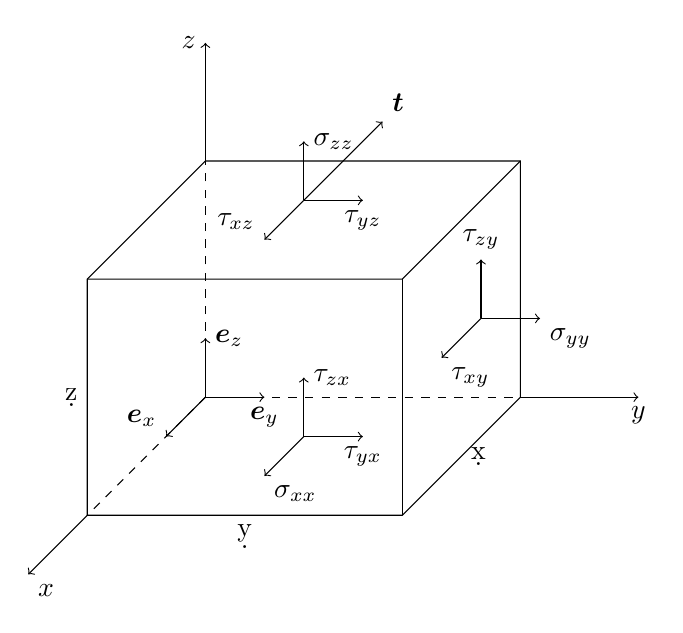
\begin{tikzpicture}
            \draw[dashed] (0,0) -- (4,0);
            \draw[->] (4,0) -- (5.5,0) node[below] {\(y\)};
            \draw[dashed] (0,0) -- (0,3);
            \draw[->] (0,3) -- (0,4.5) node[left] {\(z\)};
            \draw[dashed] (0,0) -- (-1.5,-1.5);
            \draw[->] (-1.5,-1.5) -- (-2.25,-2.25) node[below right] {\(x\)};
            \draw (-1.5,-1.5) -- (-1.5,1.5) -- (0,3) -- (4,3) -- (4,0) -- (2.5,-1.5) -- cycle;
            \draw (-1.5,1.5) -- (2.5,1.5) -- (4,3);
            \draw (2.5,1.5) -- (2.5,-1.5);
            \draw[->] (0,0) -- (-.5,-.5) node[above left] {\(\bm{e}_x\)};
            \draw[->] (0,0) -- (.75,0) node[below] {\(\bm{e}_y\)};
            \draw[->] (0,0) -- (0,.75) node[right] {\(\bm{e}_z\)};
            \draw[->] (1.25,-.5) -- (.75,-1) node[below right] {\(\sigma_{xx}\)};
            \draw[->] (1.25,-.5) -- (2,-.5) node[below] {\(\tau_{yx}\)};
            \draw[->] (1.25,-.5) -- (1.25,.25) node[right] {\(\tau_{zx}\)};
            \draw[->] (3.5,1) -- (3,.5) node[below right] {\(\tau_{xy}\)};
            \draw[->] (3.5,1) -- (4.25,1) node[below right] {\(\sigma_{yy}\)};
            \draw[->] (3.5,1) -- (3.5,1.75) node[above] {\(\tau_{zy}\)};
            \draw[->] (1.25,2.5) -- (.75,2) node[above left] {\(\tau_{xz}\)};
            \draw[->] (1.25,2.5) -- (2,2.5) node[below] {\(\tau_{yz}\)};
            \draw[->] (1.25,2.5) -- (1.25,3.25) node[right] {\(\sigma_{zz}\)};
            \draw[->] (1.25,2.5) -- (2.25,3.5) node[above right] {\(\bm{t}\)};
            \node[anchor=east] at (-1.5,0) {\(\d z\)};
            \node[anchor=north] at (.5,-1.5) {\(\d y\)};
            \node[anchor=west] at (3.25,-.75) {\(\d x\)};
        \end{tikzpicture}
    \end{center}

    Auf jeder dieser drei orthogonalen Ebenen definieren wir mithilfe von \eqref{eq:2} analog zur Schnittfläche in der vorherigen Abbildung wiederum einen Spannungsvektor, welcher sich in die Komponenten der Normal- und Schubspannung zerlegen lässt.
    Die Schubspannung wird zusätzlich in zwei weiteren Komponenten entlang der zur Schnittfläche parallelen Koordinatenachsen zerlegt.
    Die so definierten Normal- und Schubspannungskomponenten bezeichnet man beispielsweise als \(\sigma_{yy}\) bzw. \(\tau_{xy}\).
    Dabei gibt der erste Index die Richtung der Spannungskomponente an, während der zweite Index die Richtung der Flächennormale charakterisiert.
    Für die Normalspannungskomponenten stimmen diese beiden Indizes überein.
    Daher genügt es, einen Index wie folgt anzugeben
    \[
        \sigma_{xx} \to \sigma_x, \quad \sigma_{yy} \to \sigma_y, \quad \sigma_{zz} \to \sigma_z.
    \]

    Somit würde beispielhaft der Spannungsvektor auf der zur \(z\)-Richtung orthogonalen Ebene folgende Form haben
    \[
        \bm{t} = \tau_{xz}\bm{e}_x + \tau_{yz}\bm{e}_y + \sigma_z\bm{e}_z,
    \]
    wobei \(\bm{e}_x\), \(\bm{e}_y\) und \(\bm{e}_z\) die Einheitsvektoren in die entsprechenden Richtungen der Koordinatenachsen bezeichnen.

    Die Vorzeichen der oben definierten Spannungskomponenten legt man auf der Basis einer Vorzeichenkonvention wie folgt fest.
    Positive Spannungen zeigen an einem positiven (negativen) Schnittufer in die positive (negative) Koordinatenrichtung.
    Dabei spricht man von einem positiven Schnittufer wenn die Richtung der äußeren Normale mit der Richtung der entsprechenden Achse übereinstimmt.
    Genauso wie auch bei Stäben beanspruchen somit positive (negative) Normalspannungen den inifitesimalen Quader auf Zug (Druck).
    \begin{center}
        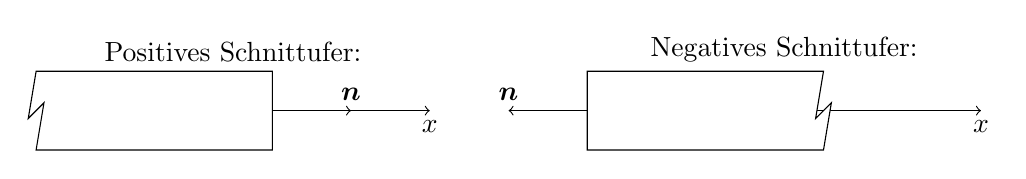
\begin{tikzpicture}
            \node[anchor=south] at (2.5,1) {Positives Schnittufer:};
            \draw (0,0) -- (.1,.6) -- (-.1,.4) -- (0,1) -- (3,1) -- (3,0) -- cycle;
            \draw[->] (3,.5) -- (5,.5) node[below] {\(x\)};
            \draw[->] (3,.5) -- (4,.5) node[above] {\(\bm{n}\)};
            \begin{scope}[shift={(7,0)}]
                \node[anchor=south] at (2.5,1) {Negatives Schnittufer:};
                \draw[->] (2.9,.5) -- (5,.5) node[below] {\(x\)};
                \draw[fill=white] (0,0) -- (0,1) -- (3,1) -- (2.9,.4) -- (3.1,.6) -- (3,0) -- cycle;
                \draw[->] (0,.5) -- (-1,.5) node[above] {\(\bm{n}\)};
            \end{scope} 
        \end{tikzpicture}
    \end{center}

    Insgesamt haben wir drei Komponenten der Normalspannung (\(\sigma_x\), \(\sigma_y\) und \(\sigma_z\)) und sechs Komponenten der Schubspannung (\(\tau_{xy}\), \(\tau_{yx}\), \(\tau_{xz}\), \(\tau_{zx}\), \(\tau_{yz}\) und \(\tau_{zy}\)) definiert.
    Man kann allerdings zeigen, dass die Schubspannungskomponenten voneinander nicht unabhängig, sondern paarweise gleich sind.
    Hierzu betrachten wir das Momentengleichgewicht um eine zur \(x\)-Richtung parallele Achse durch den Mittelpunkt des Quaders.

    % TODO: Ebener Spannungszustand

    Zur Berechnung der Kräfte müssen dabei die Spannungskomponenten mit den jeweiligen Flächeninhalten multipliziert werden.
    Die Momente ergeben sich weiterhin als Produkt der Kräfte und der entsprechenden Hebelarme.
    Somit gilt:
    \[
        M:\quad 2\frac{\d y}{2}\parentheses*{\tau_{zy}\d x\d z} - 2\frac{\d z}{2}\parentheses*{\tau_{yz}\d x\d y} = 0,
    \]
    wodurch man die Beziehung \(\tau_yz = \tau_zy\) erhält.
    Durch Bedingungen des Momentengleichgewichts um die verbleibenden Achsen erhält man schließlich
    \begin{equation}\label{eq:3}
        \tau_{xy} = \tau_{yx}, \quad \tau_{xz} = \tau_{zx}, \quad \tau_{yz} = \tau_{zy}.
    \end{equation}
    Demnach gilt: In zwei senkrecht aufeinander stehenden Ebenen sind die zur deren Schnittgeraden orthogonalen Komponenten der Schubspannungen gleich.
    Man nennt sie einander zugeordnete Schubspannungen.

    Nun kann man mithilfe von \eqref{eq:3} schlussendlich Spannungskomponenten in Form einer Matrix wie folgt darstellen
    \begin{equation}\label{eq:4}
        \brackets*{\bm{\sigma}} = \begin{bmatrix}
            \sigma_x & \tau_{xy} & \tau_{xz}\\
            \tau_{yx} & \sigma_y & \tau_{yz}\\
            \tau_{zx} & \tau_{zy} & \sigma_z
        \end{bmatrix}.
    \end{equation}
    Wegen \eqref{eq:3} ist diese Matrix, die man als Spannungsmatrix bezeichnet, symmetrisch.
    Die Größe \(\bm{\sigma}\) wird auch Spannungstensor genannt.
    Die Matrix in \eqref{eq:4} spiegelt seine Komponenten wider.
    Im Vergleich zu einer Matrix wird ein Tensor durch bestimmte Invarianten charakterisiert, die sich im Gegensatz zu den einzelnen Komponenten bei einer Transformation des Koordinatensystems nicht ändern.
    Diese Transformationen betrachten wir ausführlich in dem nächsten Abschnitt.


    \section*{Koordinatentransformation}

    Aus den im letzten Abschnitt definierten sechs Spannungskomponenten kann man nun die Spannungen in einem beliebigen schrägen Schnitt bestimmen.
    Hierzu betrachten wir ein aus der Scheibe herausgeschnittenes infinitesimales Dreieck der Dicke \(t\).
    \begin{center}
        \begin{tikzpicture}
            \draw[->] (0,0) coordinate (o) -- (6,0) coordinate(x) node [below] {\(x\)};
            \draw[->] (0,0) -- (0,3.5) node [left] {\(y\)};
            \draw (0,2.5) -- (5,0);
            \draw[->] (0,0) -- (1.5,3) coordinate(xi) node [below right] {\(\xi\)};
            \draw[->] (-.1,2) -- (-.1,1) node[left] {\(\tau_{yx}\)};
            \draw[->] (-.2,1.5) -- (-.7,1.5) node[above] {\(\sigma_x\)};
            \draw[->] (0,0) -- (-2,1) node[below] {\(\eta\)};
            \draw[->] (3,-.1) -- (2,-.1) node[below] {\(\tau_{xy}\)};
            \draw[->] (2.5,-.2) -- (2.5,-.7) node[right] {\(\sigma_y\)};
            \node[anchor=west] at (0,1.25) {\(\d y\)};
            \node[anchor=south] at (2.5,0) {\(\d x\)};
            \node[anchor=south west] at (3,1) {\(\d\eta\)};
            \draw[->] (1.5,1.85) -- (.5,2.35) node[above] {\(\tau_{\eta\xi}\)};
            \draw[->] (1.25,2.075) -- (1.5, 2.575) node[below right] {\(\sigma_\xi\)};
            \pic[draw,->,"$\varphi$",angle eccentricity=1.5] {angle=x--o--xi};
        \end{tikzpicture}
    \end{center}

    Um die Spannungen auf dem schrägen Schnitt zu definieren, führen wir ein \(\xi, \eta\)-Koordinatensystem ein, welches gegenüber dem ursprünglichen \(x, y\)-Koordinatensystem um den Winkel \(\varphi\) gegen den Uhrzeigersinn gedreht ist.
    Dementsprechend bezeichnen wir die Spannungskomponenten in der schrägen Schnittfläche mit \(\sigma_\xi\) und \(\tau_{\eta\xi}\).
    Der Flächeninhalt dieses Schnitts ergibt sich zu \(\d A = t\d\eta\).
    Die beiden anderen Schnittflächen haben die Größen \(\d A\sin\varphi\) und \(\d A\cos\varphi\).
    Die Kräftegleichgewichtsbedingungen in \(\xi\)- und \(\eta\)-Richtung nehmen somit die Form an
    \begin{align*}
        \nearrow: \quad \sigma_\xi \d A &- \parentheses*{\sigma_x \d A\cos\varphi}\cos\varphi - \parentheses*{\tau_{yx} \d A\cos\varphi}\sin\varphi\\
        &- \parentheses*{\sigma_y \d A\sin\varphi}\sin\varphi - \parentheses*{\tau_{xy} \d A\sin\varphi}\cos\varphi = 0,\\
        \nwarrow: \quad \tau_{\eta\xi} \d A &- \parentheses*{\sigma_x \d A\cos\varphi}\sin\varphi - \parentheses*{\tau_{yx} \d A\cos\varphi}\cos\varphi\\
        &- \parentheses*{\sigma_y \d A\sin\varphi}\cos\varphi - \parentheses*{\tau_{xy} \d A\sin\varphi}\sin\varphi = 0.
    \end{align*}
    Mit \(\tau_{xy} = \tau_{yx}\) aus \eqref{eq:3} ergibt sich daraus
    \begin{align}\label{eq:5}
        \sigma_\xi &= \sigma_x \cos^2 \varphi + \sigma_y \sin^2 \varphi + 2\tau_{xy}\sin\varphi\cos\varphi,\nonumber\\
        \tau_{\eta\xi} &= -\parentheses*{\sigma_x - \sigma_y}\sin\varphi\cos\varphi + \tau_{xy}\parentheses*{\cos^2 \varphi - \sin^2 \varphi}.
    \end{align}
    Es muss nur noch die Normalspannung \(\sigma_\eta\) ermittelt werden.
    Hierzu kann in der ersten Gleichung \eqref{eq:5} der Winkel \(\varphi\) durch \(\varphi' = \varphi + \frac{\pi}{2}\) ersetzt werden.
    Unter Berücksichtigung der trigonometrischen Beziehungen \(\cos\parentheses*{\varphi + \frac{\pi}{2}} = -\sin\varphi\) und \(\sin\parentheses*{\varphi + \frac{\pi}{2}} = \cos\varphi\) erhält man somit
    \[
        \sigma_\eta = \sigma_x \sin^2 \varphi + \sigma_y \cos^2 \varphi - 2\tau_{xy}\cos\varphi\sin\varphi.
    \]

    % TODO: Spannungskomponenten um gedrehten Koordinatensystem

    Mithilfe der weiteren trigonometrischen Formeln
    \begin{align*}
        \cos^2 \varphi &= \frac{1}{2}\parentheses*{1 + \cos 2\varphi}, & 2\sin\varphi\cos\varphi &= \sin 2\varphi,\\
        \sin^2 \varphi &= \frac{1}{2}\parentheses*{1 - \cos 2\varphi}, & \cos^2 \varphi - \sin^2 \varphi &= \cos 2\varphi
    \end{align*}
    werden die obigen Transformationsbeziehungen üblicherweise durch den doppelten Winkel \(\varphi\) wie folgt ausgedrückt
    \begin{align}\label{eq:6}
        \sigma_\xi &= \frac{1}{2}\parentheses*{\sigma_x + \sigma_y} + \frac{1}{2}\parentheses*{\sigma_x - \sigma_y}\cos 2\varphi + \tau_{xy}\sin 2\varphi,\nonumber\\
        \sigma_\eta &= \frac{1}{2}\parentheses*{\sigma_x + \sigma_y} - \frac{1}{2}\parentheses*{\sigma_x - \sigma_y}\cos 2\varphi - \tau_{xy}\sin 2\varphi,\\
        \tau_{\xi\eta} &= -\frac{1}{2}\parentheses*{\sigma_x - \sigma_y}\sin 2\varphi - \tau_{xy}\cos 2\varphi.\nonumber
    \end{align}
    Dies sind Transformationsgleichungen für die Komponenten des Spannungstensors.
    Wie bereits erwähnt können die Tensorkomponenten durch bestimmte Invarianten charakterisiert werden, die in jedem Koordinatensystem gleich sind.
    Für die Transformation \eqref{eq:6} gilt
    \begin{align}\label{eq:7}
        \sigma_\xi + \sigma_\eta &= \sigma_x + \sigma_y,\nonumber\\
        \sigma_\xi \sigma_\eta - \tau_{\xi\eta}^2 &= \sigma_x \sigma_y - \tau_{xy}^2.
    \end{align}
    Die Beziehung \eqref{eq:7}\({}_1\) ergibt sich beispielsweise durch Addition der ersten und zweiten Gleichung \eqref{eq:6}.
\end{document}
